\chapter{Experiments}\label{chap:experiments}

Provide numerical results, plots, and timings. Interpret the data.

Hardware and Software Used
We utilize custom-designed quadrotors that are based on 3D
printed and electronic parts of our own design, combined with
some commercial off-the-shelf components (see Fig. 1). These
platforms are lightweight (~880 grams) and safe for operation
in close proximity with humans. However, they are also agile
while maintaining maneuverability and robust vision-based
control. We have demonstrated a maximum speed of at least
4 m/s with them during vision-based flight. They are also
capable of carrying a payload of at least 200 grams in their
current configuration, but we are working to increase this
capacity. Our quadrotors are equipped with a forward-looking
global-shutter camera, an inertial measurement unit, and a
quad-core single board computer (Odroid XU4). We perform
all computations necessary for perception, state estimation,
and control onboard the quadrotor, with this computer.
Our software systems are designed in a modular way, and
utilize the Robot Operating System (ROS) for interprocess
communication. The backbone of our system is accurate state
estimation provided by our visual odometry algorithm, Semidirect
Monocular Visual Odometry (SVO) [1]. It provides a
precise and robust pose estimate, and it runs at up to 55
frames per second on the onboard embedded computer of our
flying robots. This vision-based state estimate is fused with
inertial data and gravity aligned using the Multi-Sensor Fusion
framework [2]. Because our platforms are capable of autonomous, vision-based flight utilizing only their
onboard hardware resources, they do not need to rely on external communication infrastructure to
perform their behaviors. In a field robotics scenario with uncertain communication reliability like the
MBZIRC, this is of critical importance, and our approach enables our platforms to perform their tasks
autonomously with a dependence on external communication only for high-level task coordination.

\begin{figure}[h]
   \centering
   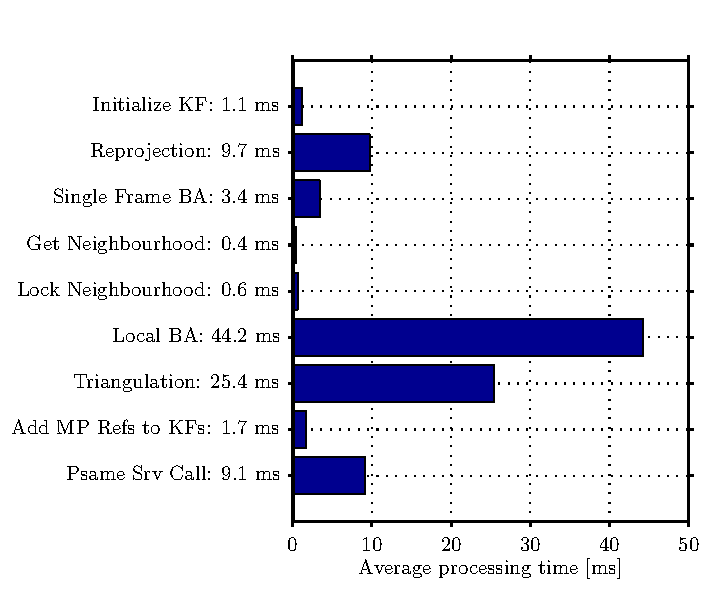
\includegraphics[width=0.75\textwidth]{img/processing_time.pdf}
   \caption{Example of a figure.}
   \label{img:timing}
\end{figure}